% ===================================================================
%  Αρχείο: 18863_tikz.tex (Fragment)
%  Αυτόματη μετατροπή μέσω doc2latex.py & TikZ conversion
% ===================================================================

ΘΕΜΑ 4

Δίνονται οι συναρτήσεις: $\varphi(x) = \sqrt{x},\ \ \text{με}\ x \geq 0$, $f(x) = \sqrt{x - 1},\ \ \text{με}\ x \geq 1$ και $g(x) = \frac{x + 1}{3},\ \ \text{με}\ x \in \mathbb{R}$.

\begin{center}
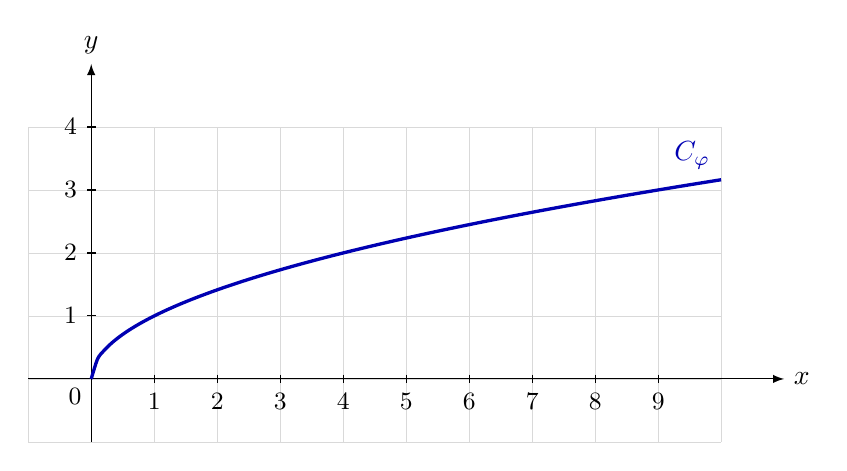
\begin{tikzpicture}[scale=0.8, >=latex]
    \draw[very thin, color=gray!30] (-1,-1) grid (10,4);
    \draw[->] (-1,0) -- (11,0) node[right] {$x$};
    \draw[->] (0,-1) -- (0,5) node[above] {$y$};
    
    \foreach \x in {1,2,3,4,5,6,7,8,9}
        \draw (\x,2pt) -- (\x,-2pt) node[below, font=\small] {\x};
    \foreach \y in {1,2,3,4}
        \draw (2pt,\y) -- (-2pt,\y) node[left, font=\small] {\y};
    \node[below left, font=\small] at (0,0) {$0$};
    
    % phi(x) = sqrt(x)
    \draw[very thick, color=blue!70!black, samples=100, smooth, domain=0:10] plot (\x, {sqrt(\x)}) node[above left] {$C_\varphi$};
\end{tikzpicture}
\end{center}

\begin{alist}
\item Να βρείτε τα κοινά σημεία των γραφικών παραστάσεων των συναρτήσεων $f$ και $g$.
\monades{08}

\item Με τη βοήθεια της γραφικής παράστασης της συνάρτησης $\varphi$, να σχεδιάσετε την γραφική παράσταση της συνάρτησης $f$.
\monades{02}

\item Στο ίδιο σύστημα συντεταγμένων, να σχεδιάσετε και την γραφική παράσταση της συνάρτησης $g$.
\monades{04}

\item Με τη βοήθεια του σχήματος ή με οποιονδήποτε άλλο τρόπο, να βρείτε το διάστημα στο οποίο η γραφική παράσταση της $f$ βρίσκεται πάνω από την γραφική παράσταση της $g$.
\monades{06}

\item Να αποδείξετε ότι $\sqrt{\ln 10 - 1} > \frac{1 + ln10}{3}$.
\monades{05}
\end{alist}
